\documentclass{article}
\usepackage[gen]{eurosym}
\usepackage{tabularx}
\usepackage{epigraph}
\usepackage{textcomp}
\usepackage[english]{babel}
\usepackage[utf8]{inputenc}
\usepackage{amsmath}
\usepackage{amsthm}
\usepackage{amssymb}
\usepackage{hyperref}
\usepackage{csquotes}% Recommended
\usepackage{rotating}
\usepackage[style=numeric]{biblatex}
% \bibliography{<mybibfile>}% ONLY selects .bib file; syntax for version <= 1.1b
\addbibresource{literature.bib}% Syntax for version >= 1.2

\usepackage{graphicx}
\graphicspath{{./00-images/}}

\usepackage{fancyhdr}
\pagestyle{fancy}
\lhead{}
\chead{}
\rhead{}
\lfoot{}
\cfoot{\thepage}
\rfoot{Property of V-Research S.r.l.}
\renewcommand\headrulewidth{0pt}
\renewcommand\footrulewidth{0pt}

\usepackage[colorinlistoftodos]{todonotes}

\newcommand{\Paragraph}[1]{\smallskip\noindent{\bf #1.}}
\newcommand{\fixnote}[2]{\textbf{\color{red}{NOTE}}\footnote{{\bf #1:} #2}}
\newcommand{\fix}[2]{{\color{red} #2}}
% \renewcommand{\fixnote}[2]{}
% \renewcommand{\fix}[2]{}

\theoremstyle{definition}
\newtheorem{definition}{Definition}[section]
\theoremstyle{corollary}
\newtheorem{corollary}{Corollary}[section]
\theoremstyle{lemma}
\newtheorem{lemma}{Lemma}[section]

\usepackage{authblk}
\date{}                     %% if you don't need date to appear
\setcounter{Maxaffil}{0}
\renewcommand\Affilfont{\itshape\small}

% for fancy table with rotated column titles
\usepackage{adjustbox}
\newcolumntype{R}[2]{%
    >{\adjustbox{angle=#1,lap=\width-(#2)}\bgroup}%
    l%
    <{\egroup}%
}
\newcommand*\rot{\multicolumn{1}{R{45}{0.01em}}}% no optional argument here, please!
\newcommand*\rota{\multicolumn{1}{R{90}{0.01em}}}% no optional argument here, please!
\def\hb{\hbox to 10.7 cm{}}

% circles
\usepackage{wasysym}
\newcommand{\Tdot}{$\CIRCLE$}
\newcommand{\Thdot}{$\LEFTcircle$}
\newcommand{\Twdot}{$\Circle$}

% formulas
\newcommand{\kframe}{K}
\newcommand{\possibleworlds}{G}
\newcommand{\modalrelation}{R}
\newcommand{\actualworld}{\omega*}
\newcommand{\world}{\omega}
\newcommand{\World}{\Omega}
\newcommand{\kmodel}{M}
\newcommand{\interpretation}{\sigma}
\newcommand{\knowledge}[1]{\mathbb{K}_{#1}}
\newcommand{\knows}[2]{K_{#1}#2}
\newcommand{\belief}[1]{\mathbb{B}_{#1}}
\newcommand{\believe}[2]{B_{#1}#2}

\makeindex 

\begin{document}

\title{On Cybersecurity\\Science and Engineering\footnote{Confidential, restricted to the authors. Property of V-Research S.r.l.}}
\author[1]{Francesco Beltramini}
\author[1]{Marco Rocchetto}
\author[2]{Luca Vigan\`o}
\affil[1]{V-Research, Verona, Italy}
\affil[2]{King's College London, UK}

\maketitle

\begin{abstract}
	The objective of this research is to develop of a theory that defines
	(all and only) the possible insecurity and security configurations of
	any abstract system. The theory is structured upon other theories that 
	defines how a component of a system can be abstracted into an agent, defining how
	agents can be formalized (both syntactically and semantically) to
	describe an abstract system, such as a graph. Some of these theories
	(e.g. used for the semantic
	definition of the abstract system) are the epistemological definition
	of knowledge, the Belief-Desire-Intent and the Assertion-Belief-Fact 
	framework of reference, 
	mereology, and topological structure. We argue that a mereology is the
	most appropriate abstract underlying structure, do to its generality,
	for defining the expressiveness of the system abstraction.  Furthermore, a
	mereology allows us to define an ontology rather than a taxonomy.  We
	also correlate different abstractions of the system to the TRL and the
	engineering V-model. 
	
	We implemented a formal theory (of axioms) of a mereotopology, and of
	the region connection calculus (RCC3 and RCC5) in a Python program that
	uses the Z3 SMT solver. The results show that a single component (i.e.
	agent) of an abstract system has a definite number of  different
	insecurity configurations (e.g. 53 using RCC5 over a topological
	structure) and only 1 secure (i.e. expected) configurations. The
	configurations are reported as models satisfying the abstract system
	semantics. 
	
	We considered the philosophical definition of truth behind our
	approach, rejecting ``proof'' by induction from partial empirical evidences.
	Our theory can be applied to system engineering and we show a concrete
	application of our theory to the risk assessment of an ad-hoc system.
	Finally, we provide a number of ideas to support the engineering of
	secure systems (e.g. purely cyber or cyber-physical).
\end{abstract}
\newpage

\section{Introduction}\label{sec:intro}
\epigraph{Humanum est errare}{{\itshape Seneca the Elder}}
The European Commission states in\autocite{EU2019market} that: ``Cybersecurity
is one of the priority areas [\ldots] of the Commission initiative on ICT
Standards, which is part of the Digitising European
Industry\autocite{EU2019standard} strategy launched on 19 April 2016.  The aim
is to identify the essential ICT standards and present measures to accelerate
their development in support of digital innovations across the economy''. The
same document (i.e.\autocite{EU2019market}) states that ``The EU will invest up
to \euro450 million [\ldots], under its research and innovation programme
Horizon 2020''. The EU, in 2016 published a press release\autocite{EU2016press}
in which they present a strategy to invest \euro1.8 \emph{billion} to
``increase measures to address cyber threats''. The EU is not the only investor
in cybersecurity, most of the developed countries and several companies are
investing enormous amount of money towards various aspects of cybersecurity
(e.g. The US vulnerability databases\autocite{NIST2020NVD} maintained by the
National Institute of Standards and Technologies, i.e. NIST, of the US
Department of Commerce).

The cybersecurity industry is growing fast, e.g. as reported
in\autocite{Nasdaq2018market}. For example, in\autocite{Forbes2017market},
published by the Forbes, is stated that \euro5.3 billion of funding where
poured by venture capitalist into cybersecurity companies in 2018. The Forbes,
in the same article, also highlights another peculiar (as seemly contradictory)
trend: ``[\ldots] during the same time period, the number of cybersecurity
breaches increased exponentially''. The data reported by the NIST 
through the official CPE (Common Platform Enumeration) Dictionary Statistics 
on the NVD websites in \autocite{NIST2020CPEstatistics}, show that in 2016 the
number of reported vulnerabilities reported where around $~6000$ while in 2019
the number of vulnerabilities was above $16000$.  The scientific community also
reports similar findings.  In fact, in\autocite{Herley2009so}, Cormac Herley
(Microsoft Research) shows how basic cybersecurity principles (such as the
confidentiality benefit over the clear text for passwords typed into forms,
e.g. for logins in websites) are not fully understood or shared between the
cybersecurity research community\autocite{Nielsen2009stop}.  The lack of
understanding of basic security principle, the inverse proportionality between
investments in cybersecurity and the number of reported vulnerabilities year
after year, can be linked to the lack of a foundational theory on
cybersecurity, as already highlighted by Cormac Herley
in\autocite{Herley2016unfalsifiability}. 

In this article, we give the first scientific theory (to the best of our knowledge)
on security.

\Paragraph{Structure} In Section~\ref{sec:problem} we define and formalize the problem statement. 
In Section~\ref{sec:theory} we outline our security theory, and in Section~\ref{sec:prototest}
we describe the implementation of the theory and some empirical tests of the theory.
Finally, in Section~\ref{sec:related} we conclude the paper with an overview of the related work.


\section{Problem Statement}\label{sec:problem}

\begin{figure}[t]
	\centering
	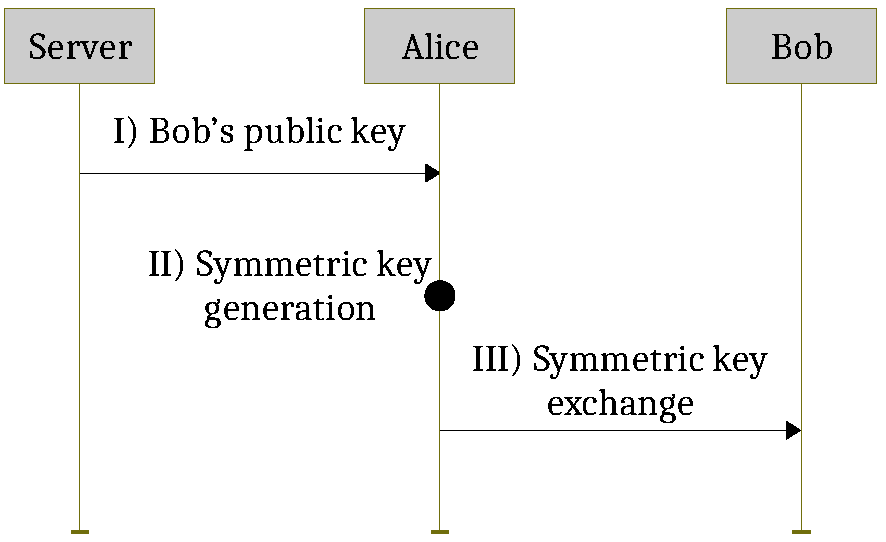
\includegraphics[width=.6\textwidth]{protocol-example.pdf}
	\caption{Abstraction of an ad-hoc esemplificative protocol execution}
	\label{fig:protocol-example}
\end{figure}

In\autocite{Herley2016unfalsifiability}, Cormac Herley explores what he calls
``an asymmetry in computer security'', which he defines as follows: ``Things
can be declared insecure by observation, but not the reverse. There is no
observation that allows us to declare an arbitrary system or technique
secure''. Herley then uses this argument to show that ``claims that any measure
is necessary for security are empirically unfalsifiable''. Given that, any
theory which is not falsifiable by an empirical experiment is well
known\footnote{``A theory which is not refutable by any conceivable event is
nonscientific. Irrefutability is not a virtue of a theory (as people often
think) but a vice.'' -- Karl Popper, Conjectures and
Refutations\autocite{popper1962conjectures}} to be nonscientific (i.e.
unfalsifiability is a fallacy of a theory), Herley concludes that there is no
scientific theory on cybersecurity; which means that cybersecurity lays in the
realm of pseudo-sciences\autocite{Herley2016usenixvideo}.  Herley, e.g.
in\autocite{Herley2017justifying}, discusses the implications of a
nonscientific approach to cybersecurity, and highlights the tremendous impact on
all the scientific research and engineering of systems; leading often to
terrorism and wars, and wasting of resources in useless protections or
overspending.  While the criticism is investigated
in\autocite{Herley2016unfalsifiability}, no solution is provided.  On the
contrary, the goal of this work \emph{is} to lay the foundations of a
scientific cybersecurity theory. Furthermore, in Section~\ref{sec:sicurezza},
we consider the problem raised by Herley not confined to ``computer security''
but to any abstract system (so that our theory may hold for any sound
implementation such as networks, mechanical, cyber, or cyber-physical system,
or even a single computer or a single device such as an hard-drive).  There is
also an apparent inconsistency in\autocite{Herley2016unfalsifiability} that we
seek to clarify before following (as we agree) the scientific path draw by
Herley: cybersecurity is defined as an abstract property in many formal
approaches to the investigation of the security of systems, and the security of the design of a
formally verified protocol is indeed falsifiable.  For example, in the protocol
verification community, security is often defined as a formalization of the
high-level properties confidentiality, integrity, and availability. The problem
in such approaches is not the definition of what cybersecurity is, but the use
of theories (such as the Dolev-Yao attacker model\footnote{For the sake of
simplicity, the Dolev-Yao attacker can be considered as an abstraction of an
active attacker who controls the network but cannot break
cryptography.}\autocite{Dolev1983security})
that only applies to specific instances (often called scenarios) and
abstraction of the protocol. This, in turn, creates a false sense of security
since requires assumptions on the abstraction of the system of which security
is verified. As an example, for the formal security verification of the system
in Figure~\ref{fig:protocol-example}, a formalized scenario needs to be defined
by a modeler who chooses (among others): (i) a scope of the formalization (e.g.
excluding the server that distributes the public key is often done when
verifying the security of authentication protocols), (ii) the number of
sessions (even tough some approaches do reason on an infinite number of
sessions such as\autocite{Escobar2007maudenpa}), (iii) honesty/dishonesty of
the peers (e.g.  in the ASLan++ language\autocite{Oheimb2010aslan++}), and (iv)
the abstraction of the cryptographic primitives (e.g.  ProVerif vs
CryptoVerif\autocite{Blanchet2017symbolic}).  Some of the choices will
completely change the results of the formal verification of the system. For
example, under the perfect cryptography assumption\footnote{As defined
in\autocite{Rocchetto2016cpdy}: ``In the so called perfect cryptography
assumption, the security encryption scheme is suppose to be perfect, without
any exploitable flaw, and so the only way for the attacker to decrypt a message
is by using the proper key. That assumption is widely accepted in the security
protocol community, and most of the formal reasoning tools for the analysis of
security protocols abstract away the mathematical and implementation details of
the encryption
scheme\autocite{Turuani2006clatse,Basin2005ofmc,Armando2016satmc,Rocchetto2017interpolation}''}
and assuming that no violation to any security property is done after message
I); in Figure~\ref{fig:protocol-example}, the freedom of choosing the scope
determines that the flaws related to the dishonest impersonation of the Server
may or may not be considered in the verification process.  This choice has
tremendous impact on the focus and findings of the verification of the security
of the protocol.  While this may seem to turn upon minutiae and foreseeable,
this highlights the false sense of security that may derive from a
non-scientific theory of system security\footnote{``To the superficial
observer, the analysis of these forms seems to turn upon minutiae. It does in
fact deal with minutiae, but they are of the same order as those dealt with in
microscopic anatomy.'' -- Karl Marx, Capital Volume 1, 1867}.

\subsection{Sicurezza: Safety and Security}\label{sec:sicurezza}
In most of the natural languages, and in Italian too, the concepts of safety
and security are not syntactically differentiated and both terms (safety and
security) are expressed by the same word, e.g. sicurezza in Italian.  A
semantic distinction between safety and security is correlated to a
belief\footnote{A belief has to be intended as a proposition which is supposed
to be true by the majority of humans in our society without a scientific
underlying theory but based on partial empirical evidences or inductive proofs.} that
safety deals with \emph{accidents} (i.e. an unfortunate incident) posed by the
natural environment (e.g. natural events such as wearing of hardware
components) while security deals with \emph{incidents} posed by mankind (e.g.
attackers and bugs).  The fundamental difference between nature and mankind (and,
in turn, between safety and cybersecurity) is believed to be on the different
intents\footnote{``The belief–desire–intention software model (BDI) is a
software model developed for programming intelligent
agents.''\autocite{wiki-bdi}. In the BDI model, the intents represents the
deliberative state of an agent which determines the choice of that agent on
what to do.} (accidents are unfortunate while incidents are not) of the causes
that generates the threat; namely, nature is believed not to have malicious
intents (but unfortunate causes-effects) while threats generated by mankind are
believed to be malicious\footnote{Of course, logical flaws or bugs may be
introduced by other means (e.g. ignorance) without explicit malicious intents,
but the exploitation of those flaws is considered (for now, and detailed
afterwards in the article) malicious, and then we consider any vulnerability to
be malicious (without loss of generality) even if due to the lack of skills.}.
An overview on the aforementioned aspects of safety and security is depicted in
Figure~\ref{fig:safety-security} and is used as a baseline for a definition of
the terms that structure our current understanding of safety and security. 
\begin{itemize}
	\item \emph{Mankind} ``refers collectively to humans''
\autocite{wiki-mankind}, while the concept of \emph{Nature} is
		related ``to the intrinsic characteristics that plants,
		animals, and other features of the world develop of their own
		accord'' (e.g. the physical universe)\autocite{wiki-nature}. 
		\begin{itemize}
			\item So far, we have used several terms to refer to an
				\emph{attacker}, i.e. threat agent or threat source,
				considering those terms to be semantically
				equivalent.  This ``shallowness'' raise form the
				necessity of properly citing the different sources, but,
				in the reminder of this paper, we consider the
				Causality principle to be the \emph{threat
				source}, Nature or Mankind to be the
				\emph{threat agents} and an \emph{attacker} as
				a specific malicious threat agent which materialize a
				threat.
		\end{itemize}
	\item \emph{Vulnerability}\footnote{The term vulnerability is not
		present in the Encyclopedia of Cryptography and Security, while
		it is used in 12 entries (such as in the definition of
		``penetration testing''\autocite{caddy2005pentest})
		highlighting how commonly this word is used without a proper
		supporting semantics}, as defined in\autocite{cnssi20104009}
		(and adopted in\autocite{nist2013800-53}), is ``weakness in an
		information system, system security procedures, internal
		controls, or implementation that could be exploited by a threat
		source''. On the one hand, the definition is broad to enclose
		as much causes (that generates a vulnerability) as possible; on
		the other hand, it derives from empirical evidences (which
		should be considered beliefs\footnote{``For this view, that
		\emph{That Which Is Not} exists, can never predominate. You
		must debar your thought from this way of search, nor let
		ordinary experience in its variety force you along this way,
		(namely, that of allowing) the eye, sightless as it is, and the
		ear, full of sound, and the tongue, to rule; but (you must)
		judge by means of the Reason (Logos) the much-contested proof
		which is expounded by me.'' -- Parmenides of Elea, On Nature
		(circa 500 B.C.), fragments B7.1–8.2
		\autocite{Hakim2016philosophy}} since they are partial results in nature) 
		while a vulnerability should
		be defined in a way that is empirically falsifiable. This means
		that the term vulnerability should have a complete and sound
		definition, so that no other causes (e.g.  other sources) but
		the ones in the definition are responsible for a vulnerability.
		Furthermore, the term ``threat sources'' used in the definition
		in\autocite{cnssi20104009} may be identified with both Nature
		and Mankind, not differentiating between safety and security.
		In Definition~\ref{def:vulnerability}, we provide a formal
		theory of vulnerability (so that the scientific community can
		identify tests for the completeness and soundness of the
		definition itself).
\end{itemize}

\begin{figure}[t]
	\centering
	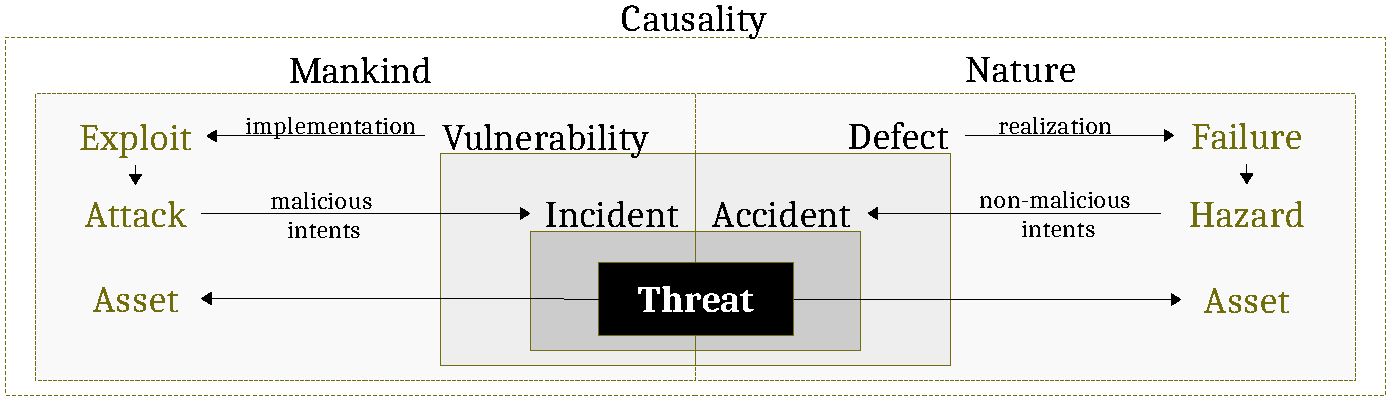
\includegraphics[width=\textwidth]{safety-security.pdf}
	\caption{Overview security and safety keywords}
	\label{fig:safety-security}
\end{figure}

Most of the safety-preserving principles in the field of engineering of
safety-critical cyber-physical systems (such as elevators and aircraft), upon
which safety requirements (e.g. in standards such as the IEC 61508 or 61511\autocite{IEC201761511}) are defined, have
been defined following empirical tests and measurements. While reasoning by
induction based on the empirical observation should be avoided, since it may
easily lead to false beliefs instead of scientific theories, this approach is
often justified by the supposed impossibility of defining a theory that
correctly predicts failures which, in turn, pose hazards to a system. 
To the best of our knowledge, and supported by\autocite{Herley2016unfalsifiability}, the
correlation between predictability of environment and believed unpredictability
of attackers (i.e. a malicious
environment) has not been correlated to a theory on cybersecurity. 
Therefore, inductive research efforts in
predicting malicious effects are accepted (and published) in scientific
conferences (e.g.~\autocite{Rocchetto2014CSRF}). A failure of a wire due to
environment (e.g. due to humidity, dust, heat \&c) is defined from empirical
evidences and processes have been standardized to test qualities of hardware components
%convinced by the induction principle. What is already a
%weak argument in general, 
This process completely breaks down when a malicious environment (i.e. an attacker)
is considered instead of the (supposedly honest and predictable)
natural environment. Therefore, the same approach that is in use for safety,
seems not to be applicable to test security.

Going back to Figure~\ref{fig:safety-security}, a vulnerability does not
necessarily become a threat for the system, unless exploited ``through a
channel that allows the violation of the security policy
[\ldots]''\autocite{cnssi20104009} (e.g. a software or procedure) that takes
advantage of the vulnerability causing an \emph{attack} to the system, which may
result in several correlated incidents and threats.  The process of
exploitation of a defect as a vulnerability is reported in
Figure~\ref{fig:safety-security} such that the difference between exploit and failure,
and attack and accident is to be found just in the maliciousness of the intents
that causes this process (i.e. excluding the intent, the terms are just syntactic transformation from a vulnerability to defect, from
accident to incident). In the following, we conclude the informal definition of
the terms that we used in this section and in Figure~\ref{fig:safety-security}.

\begin{itemize}
	\item \emph{Causality} refers to the causality principle; defined
		in\autocite{Spirkin1983Dialectical} as ``Causality is a genetic
		connection of phenomena through which one thing (the cause)
		under certain conditions gives rise to, causes something else
		(the effect). The essence of causality is the generation and
		determination of one phenomenon by another. In this respect
		causality differs from various other kinds of connection, for
		example, the simple temporal sequence of phenomena, of the
		regularities of accompanying processes''.
	\item An \emph{Exploit}\footnote{We note that the term exploit is only
		used as a verb in\autocite{ISO2009information}} is ``An exploit
		(from the English verb to exploit, meaning to use something to
		one’s own advantage) is a piece of software, a chunk of data,
		or a sequence of commands that takes advantage of a bug or
		vulnerability to cause unintended or unanticipated behavior to
		occur on computer software, hardware, or something electronic
		(usually computerized).''\autocite{wiki-exploit}.
	\item An \emph{Attack}, as defined by the International Standard
		ISO/IEC 27000 is an ``attempt to destroy, expose, alter,
		disable, steal or gain unauthorized access to or make
		unauthorized use of an asset''; where an \emph{Asset} is
		``anything that has value to the organization''. We note that for
		the purpose of this article, we do not want to focus on a specific
		organization or business to define asset but, in general, on any 
		abstract organization (e.g. a company or a society).
		We do not consider ethical hackers as attacking a system. 
		In fact, we consider the term \emph{hack} as
		non-malicious (see Hacker\autocite{Stallman2002hacker}).
	\item A \emph{Threat}, as defined in\autocite{cnssi20104009}, is ``Any
		circumstance or event with the potential to adversely impact
		organizational operations (including mission, functions, image,
		or reputation), organizational assets, individuals, other
		organizations, or the Nation through an information system via
		unauthorized access, destruction, disclosure, modification of
		information, and/or denial of service''.
	\item \emph{Defect}, ``anything that renders the product not reasonably
		safe''\autocite{Robinson2019writing} (i.e. a characteristic of
		an object which hinders its proper usability).
	\item \emph{Failure}, as defined in\autocite{Merriam2020failure} as ``a state of
		inability to perform a normal function''. The term is
		structured and detailed in
		\autocite{cnssi20104009,iet2017glossary} but relying on an
		abstract notion of failure without a specific definition.
	\item \emph{Hazard}, ``a potential source of
		harm''\autocite{iet2017glossary}.
\end{itemize}

\printbibliography

\end{document}
